% !TeX root = ../../../book.tex

\subsection{关于像的证明}

你可能已经通过研究先前的一些例子发现了此性质。但我们仍需通过使用像的定义来陈述和证明该命题。请注意,这是关于\emph{任意}函数的命题;无论 $f$ 是什么,它都成立!

\begin{proposition}\label{prop:proposition7.3.6}
    设 $A, B$ 为集合,$f:A \to B$ 为函数。若 $S, T \subseteq A$,则
    \[\im_f (S \cap T) \subseteq \im_f (S) \cap \im_f (T)\]
\end{proposition}

\begin{proof}
    设 $z \in \im_f (S \cap T)$ 为任意固定元素。这意味着 $\exists a \in S \cap T$ 使得 $f(a) = z$。
    
    给定这样的 $a$。由 $a \in S \cap T$ 可知 $a \in S$ 且 $a \in T$。

    因此,根据像的定义,$z \in \im_f (S)$ 且 $z \in \im_f (T)$。

    根据交集的定义,可推导出 $z \in \im_f (S) \cap \im_f (T)$。

    这证明了待证的集合包含关系。
\end{proof}

为什么我们没有在这里声明\emph{相等}呢?实际上,相等\emph{并不总是成立}。也就是说,存在至少一个函数使得反向包含关系 $\im_f(S) \cap \im_f(T) \subseteq \im_f(S \cap T)$ 不成立。我们将在下文提供这样一个函数的例子。

(尝试构造一个反向包含关系\emph{成立}的函数例子。这样就能证明该包含关系并非\emph{必然}成立!)

我们将通过示意图展示一个具有特定性质的例子。然后,我们会正式\emph{定义}这个函数,并说明其性质,指出这些性质如何支持我们的论点。

需要注意的是,使用这种方法是完全可行的,只要你之后补充正式的定义。仅仅依靠示意图作为``证明''是不够严谨的,但它确实能帮助你构思证明的\emph{思路}。

此外,在这种情况下,没有必要构造\emph{复杂}或\emph{有趣}的反例。要\emph{反驳}一个全称量化陈述,只需\emph{一个}有效的例子即可。特别是,不必定义一个通过公式处理数字的函数,因为有时这反而会增加难度。通常,反例可以通过只包含少数元素(如两个或三个)的集合来构造。\\

\begin{example}
    我们声称存在集合 $A,B,S,T$ 和函数 $f : A \to B$,使得 $\im_f (S) \cap \im_f (T) \nsubseteq \im_f (S \cap T)$。下面构造这样的例子。基于前述讨论,尝试构造一个包含三个元素的集合,令 $A = \{1, 2, 3\}$ 并定义 $f(1) = \bigstar$。

    \begin{center}
        {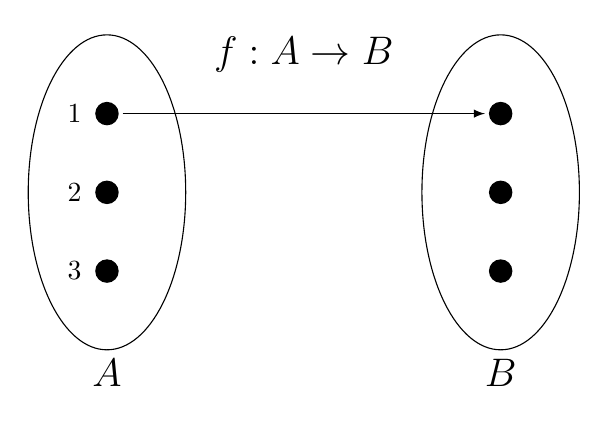
\begin{tikzpicture}[scale=1]
            \foreach \x in  {1,2,3}
            {
                \node at (5, -\x)[circle,fill,inner sep=3pt]{};
            }
            \draw[shift={(5.2, -1)}] node[right] {$\bigstar$};
            \draw (5,-2) ellipse (1 and 2);
    
            \foreach \x in  {1,2,3}
            {
                \node at (0, -\x)[circle,fill,inner sep=3pt]{};
                \draw[shift={(-0.2, -\x)}] node[left] {$\x$};
            }
            \draw (0,-2) ellipse (1 and 2);
    
            \draw[-latex] (0.2,-1) -- (4.8,-1); 
            
            \node[below] at (0, -4){\Large $A$};
            \node[below] at (5, -4){\Large $B$};
            \node[above] at (2.5, -0.6){\Large $f:A \to B$};
        \end{tikzpicture}}
    \end{center}

    为了便于定义,设 $S$ 包含两个元素 $S = \{1, 2\}$ 且 $f(1) \ne f(2)$,否则 $\im_f(S)$ 仅包含一个元素,无法体现 $S$ 的双元素特性,因此定义 $f(2) = \square$ 且 $\square \neq \bigstar$。

    \begin{center}
        {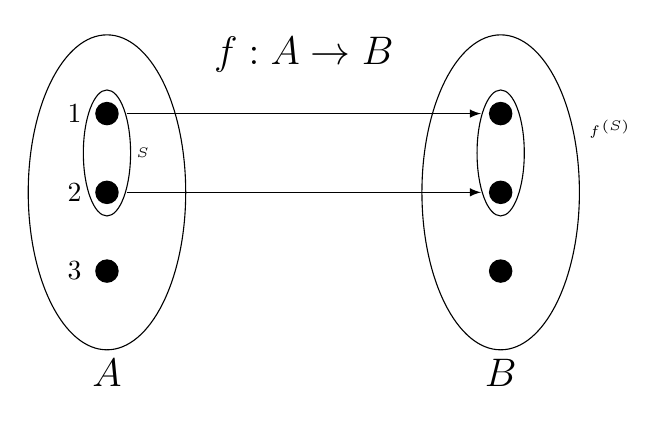
\begin{tikzpicture}[scale=1]
            \foreach \x in  {1,2,3}
            {
                \node at (5, -\x)[circle,fill,inner sep=3pt]{};
            }
            \draw[shift={(5.2, -1)}] node[right] {$\bigstar$};
            \draw[shift={(5.2, -2)}] node[right] {$\square$};
            \draw (5,-2) ellipse (1 and 2);
            \draw (5,-1.5) ellipse (0.3 and 0.8);
    
            \foreach \x in  {1,2,3}
            {
                \node at (0, -\x)[circle,fill,inner sep=3pt]{};
                \draw[shift={(-0.2, -\x)}] node[left] {$\x$};
            }
            \draw (0,-2) ellipse (1 and 2);
            \draw (0,-1.5) ellipse (0.3 and 0.8);
    
            \draw[-latex] (0.25,-1) -- (4.75,-1);
            \draw[-latex] (0.25,-2) -- (4.75,-2); 
    
            \node[right] at (0.25, -1.5){\tiny $S$};
            \node[right] at (6.0, -1.2){\tiny $\im_f(S)$};
            \node[below] at (0, -4){\Large $A$};
            \node[below] at (5, -4){\Large $B$};
            \node[above] at (2.5, -0.6){\Large $f:A \to B$};
        \end{tikzpicture}}
    \end{center}

    现在,我们需要选择集合 $T$。若令 $S \cap T = \varnothing$ 或 $T \supseteq S$ 可能引发复杂情况,故取 $T = \{2, 3\}$。接下来定义 $f(3)$,请结合示意图思考映射关系:

    \begin{itemize}
        \item 若 $f(3) = f(2) = \square$。\\
            在此情况下,$\im_f(T) = \{\square\}$,所以 $\im_f (S) \cap \im_f (T) = \{\square\} = \im_f (S \cap T)$,这行不通。
        \item 若 $f(3)$ 等于其他值,比如 $\smiley{}$。\\
            这也行不通。我们会得到 $\im_f (S) \cap \im_f (T) = \{\square\} = \im_f (S \cap T)$。
        \item 若 $f(3) = f(1) = \bigstar$。\\
            此时满足要求。
    \end{itemize}

    \begin{center}
        {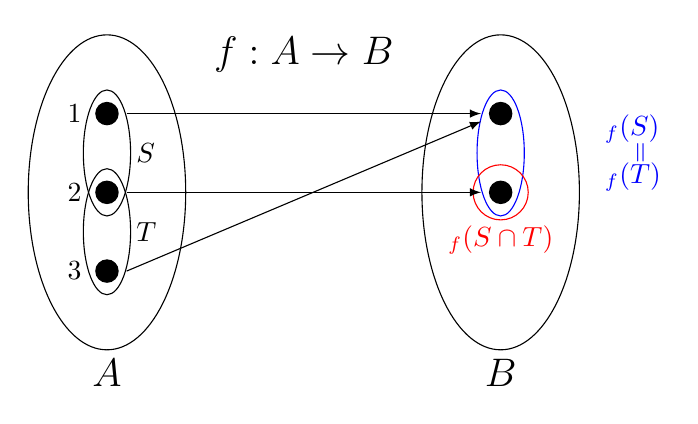
\begin{tikzpicture}[scale=1]
            \foreach \x in {1,2}
            {
                \node at (5, -\x)[circle,fill,inner sep=3pt]{};
            }
            \draw[shift={(5.2, -1)}] node[right] {$\bigstar$};
            \draw[shift={(5.2, -2)}] node[right] {$\square$};
            \draw (5,-2) ellipse (1 and 2);
            \draw[blue] (5,-1.5) ellipse (0.3 and 0.8);
            \draw[red] (5,-2) circle (0.35);
            \node[below, red] at (5, -2.3){$\im_f(S \cap T)$};
    
            \foreach \x in  {1,2,3}
            {
                \node at (0, -\x)[circle,fill,inner sep=3pt]{};
                \draw[shift={(-0.2, -\x)}] node[left] {$\x$};
            }
            \draw (0,-2) ellipse (1 and 2);
            \draw (0,-1.5) ellipse (0.3 and 0.8);
            \draw (0,-2.5) ellipse (0.3 and 0.8);
    
            \draw[-latex] (0.25,-1) -- (4.75,-1);
            \draw[-latex] (0.25,-2) -- (4.75,-2); 
            \draw[-latex] (0.25,-3) -- (4.75,-1.1); 
    
            \node[right] at (0.25, -1.5){$S$};
            \node[right] at (0.25, -2.5){$T$};
            \node[right, blue] at (6.2, -1.2){$\im_f(S)$};
            \node[right, blue, anchor=center, rotate=90] at (6.8, -1.5){$=$};
            \node[right, blue] at (6.2, -1.8){$\im_f(T)$};
            \node[below] at (0, -4){\Large$A$};
            \node[below] at (5, -4){\Large$B$};
            \node[above] at (2.5, -0.6){\Large $f:A \to B$};
        \end{tikzpicture}}
    \end{center}
\end{example}

我们已经成功构造出 $\im_f (S) \cap \im_f (T)$ 是 $\im_f (S \cap T)$ 的\emph{真}超集。

回顾我们的构造过程,看看你是否理解我们的思路。我们需要遵守哪些限制?在哪些方面有选择的自由?我们最终是如何决定的?

需要说明的是,这绝对不是\emph{唯一的}例子!你也可以尝试构造其他反例。

现在,我们只需用最终构造出的示意图定义一个实例,并证明其有效性。开始吧!

\begin{proof}
    定义 $A = \{1, 2, 3\}, B = \{\bigstar, \square\}$。

    定义 $f : A \to B$ 为 $f(1) = \bigstar, f(2) = \square, f(3) = \bigstar$。

    定义 $S = \{1, 2\}, T = \{2, 3\}$。

    易得 $S \cap T = \{2\}$,所以 $\im_f (S \cap T) = \{f(2)\} = \{\square\}$。

    然而,$\im_f (S) = \im_f (T) = B$,所以 $\im_f (S) \cap \im_f (T) = \{\bigstar, \square\} \ne \{\square\}$。

    由于 $\bigstar \in \im_f (S) \cap \im_f (T)$ 而 $\bigstar \notin \im_f (S \cap T)$,结论得证。
\end{proof}

我们已经展示了如何\textbf{证明}关于任意函数和像的命题,以及如何通过\textbf{构造}具体反例来\textbf{反驳}一个声明。在后续练习中,你会遇到类似问题。有时需要自行判断命题的真伪(此处我们提前指明了正确答案)。建议尝试以下两种方法:
\begin{enumerate}[label=(\arabic*)]
    \item 尝试证明该声明,观察是否会在某个步骤出现矛盾;
    \item 尝试构造反例,检验是否会遇到障碍。
\end{enumerate}
如果完成上述任意一项……恭喜,你已经解决了这个问题!如若遇到困难,这可能有助于你更深入地理解问题本质。

接下来给你布置一个具体任务:请用 ``$\cup$'' 替换 ``$\cap$'' 重新检验上述命题。你认为结果会不同吗?动手试试吧!
